\documentclass[border=6pt]{standalone}
\usepackage{pgfplots}
\pgfplotsset{compat=1.17}
\begin{document}
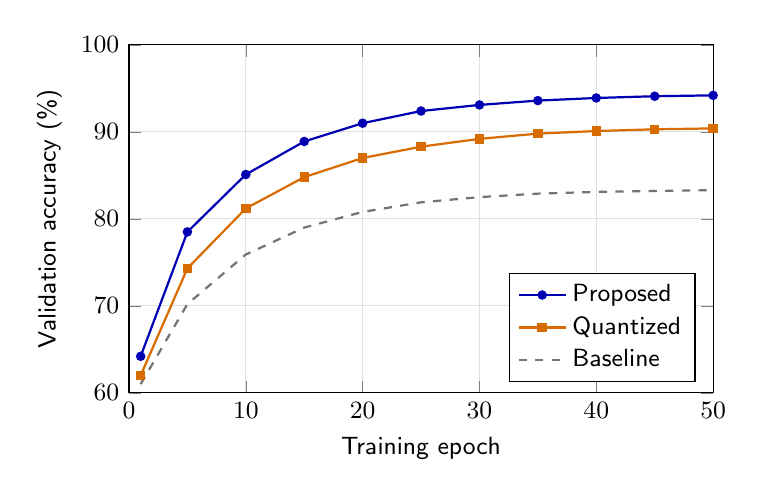
\begin{tikzpicture}
\begin{axis}[width=9cm, height=6cm, font=\sffamily\small, xlabel={Training epoch}, ylabel={Validation accuracy (\%)},
  xmin=0, xmax=50, ymin=60, ymax=100, grid=major, grid style={black!12}, legend pos=south east, legend cell align=left,
  every axis plot/.append style={thick}]
  \addplot[blue!70!black, mark=*, mark size=1.3pt] coordinates {(1,64.2)(5,78.5)(10,85.1)(15,88.9)(20,91.0)(25,92.4)(30,93.1)(35,93.6)(40,93.9)(45,94.1)(50,94.2)};
  \addplot[orange!85!black, mark=square*, mark size=1.3pt] coordinates {(1,62.0)(5,74.3)(10,81.2)(15,84.8)(20,87.0)(25,88.3)(30,89.2)(35,89.8)(40,90.1)(45,90.3)(50,90.4)};
  \addplot[black!55, dashed] coordinates {(1,61.0)(5,70.2)(10,75.9)(15,79.0)(20,80.8)(25,81.9)(30,82.5)(35,82.9)(40,83.1)(45,83.2)(50,83.3)};
  \legend{Proposed, Quantized, Baseline}
\end{axis}
\end{tikzpicture}
\end{document}
